%!TEX program = lualatex

\documentclass[12pt,a4paper,oneside]{report}
\usepackage[spanish]{babel}
\selectlanguage{spanish}
\usepackage[T1]{fontenc}
\usepackage{times}
\usepackage[utf8]{inputenc}
\usepackage{amsmath}
\usepackage{graphicx}
\usepackage{multicol}
\usepackage{longtable}
\usepackage[refpages]{gloss}
\usepackage{float}
\usepackage{anysize}
\usepackage{bigstrut}
\usepackage{appendix}
\usepackage{lscape} 
\usepackage{pdflscape}
\usepackage{multirow}
\usepackage{listings}
\usepackage{color}
\usepackage{setspace}
\usepackage{enumerate} 
\usepackage{ragged2e}
\usepackage[utf8]{inputenc}
\usepackage{comment}
\usepackage{pslatex}
\usepackage[colorlinks=true, citecolor=blue, urlcolor=blue]{hyperref}  % activa enlaces en apacite
\usepackage{apacite} 
\usepackage{fixltx2e}
\usepackage{caption}
\usepackage{setspace} 
\captionsetup[table]{skip=10pt}
\bibliographystyle{apacite}

% new packages
\usepackage{tabularx}
\usepackage{array} 
\usepackage{enumitem}

% configuracion de sangria y espacio entre párrafos
\setlength{\parskip}{1em}
\setlength{\parindent}{1.27cm}



\begin{document}
\renewcommand{\BOthers}[1]{et al.\hbox{}}
\renewcommand\bibname{Bibliografía}



%----------------------------------------------------------------------------------------
%	CONFIGURACION
%----------------------------------------------------------------------------------------
\marginsize{3.0cm}{3.0cm}{3.0cm}{3.0cm}
\renewcommand*{\contentsname}{Índice}
\renewcommand*{\listfigurename}{Lista de figuras}
\renewcommand*{\listtablename}{Lista de tablas}
\renewcommand{\baselinestretch}{1.0}
\renewcommand{\appendixname}{Anexos}
\renewcommand{\appendixtocname}{Anexos}
\renewcommand{\appendixpagename}{Anexos}
\renewcommand{\thetable}{\arabic{chapter}.\arabic{table}}
\renewcommand*{\tablename}{Tabla}
\renewcommand*{\chaptername}{Capítulo}
\renewcommand*{\thechapter}{\Roman{chapter}}
\renewcommand{\thesection}{\arabic{chapter}.\arabic{section}}
\renewcommand{\figurename}{Figura}
\renewcommand{\thefigure}{\arabic{chapter}.\arabic{figure}}
\renewcommand{\theequation}{\arabic{chapter}.\arabic{equation}}

%----------------------------------------------------------------------------------------
%	Carátula
%----------------------------------------------------------------------------------------

\begin{titlepage}
\begin{center}
    { \large UNIVERSIDAD NACIONAL DE SAN AGUSTÍN DE AREQUIPA}\\
    \vspace{4mm} 
    {\large FACULTAD DE INGENIERÍA DE PRODUCCIÓN Y SERVICIOS}\\
    \vspace{4mm} 
    {\large ESCUELA PROFESIONAL DE CIENCIA DE LA COMPUTACIÓN}\\
    
    \vspace{1.5cm}
    
    \begin{figure}[H]
        \centering
        
\includegraphics[scale=0.3]{imagenes/ESCUDO.jpg}
    \end{figure}
    
    %\vspace{0.5cm}

    %\title{Título de mi tesis} % titulo de tu tesis para latex
    \begin{spacing}{1.5}
    {\large \bf EVALUACIÓN DE LA CALIDAD SEMÁNTICA DE\\ 
    TRADUCCIONES AUTOMÁTICAS QUECHUA-ESPAÑOL AL\\
    APLICAR DISTINTOS MODELOS DE TRADUCCIÓN}\\ % titulo de tu tesis para latex
    \end{spacing}
    
    \vspace{0.5cm}
    
    \begin{spacing}{1.5}
        \makebox[7cm][l]{Tesis presentada por el Bachiller:}\\
        \makebox[7cm][l]{\textmd{\textbf{Jenny Huanca Anquise}}.}\\
        \makebox[7cm][l]{Para optar el Título de:}\\
        \makebox[7cm][l]{Licenciado en Ciencias de la Computación }\\
                
        \vspace{0.2cm}
        \makebox[7cm][l]{\textbf{Asesor:}}\\
        \makebox[7cm][l]{\textbf{Mag. Wilber R. Ramos Lovón}}
    
    \vspace{0.5cm}
    {Arequipa - Perú\\
    2025}
    \end{spacing}
    
\end{center}
\end{titlepage}

\pagenumbering{roman}
\newpage
%----------------------------------------------------------------------------------------
%	Resumen
%----------------------------------------------------------------------------------------

\chapter*{\centering \huge Resumen} 
\addcontentsline{toc}{chapter}{Resumen} % si queremos que aparezca en el índice
\markboth{Resumen}{Resumen} % encabezado

Esta investigación evalúa la calidad semántica de traducciones automáticas (TA) para el par quechua-español, analizando tres modelos: Google Translate (Transformer multilingüe), MarianMT (especializado en lenguas de bajos recursos) y un baseline léxico. El estudio surge ante la brecha digital que afecta a 8 millones de hablantes de quechua, quienes carecen de herramientas de TA confiables que preserven su riqueza lingüística y cultural. Se emplea un enfoque multimodal que combina: 1) métricas cuantitativas (similitud coseno con embeddings LaBSE, COMET-QE y chrF++) para medir equivalencia conceptual, y 2) evaluación humana por hablantes nativos que califican fluidez y adecuación cultural mediante escalas Likert.

El corpus de estudio utiliza textos del dominio educativo y narrativo oral del dataset Monolingual Quechua IIC, centrado en variantes sureñas y centrales del quechua. Los resultados preliminares indican que MarianMT supera en 18.7\% a Google Translate en preservación de sufijos evidenciales (*-mi*, *-si*), pero ambos muestran errores críticos en términos culturales como ``ayn'' (traducido como ``ayuda'' en 63\% de casos), evidenciando limitaciones en equivalencia pragmática. La evaluación humana revela que el baseline léxico logra mayor adecuación semántica para léxico cultural (+22\%), aunque con baja fluidez gramatical.

Las contribuciones centrales son: 1) Validación de métricas innovadoras (LaBSE, COMET-QE) como alternativas a BLEU para lenguas aglutinantes, mostrando correlación de 0.78 con evaluaciones humanas; 2) Generación de un dataset abierto con 500 pares de traducciones anotadas por hablantes nativos; y 3) Criterios prácticos para selección de modelos según dominios (ej: MarianMT para educación formal, baseline para narrativa cultural). Estos hallazgos benefician directamente a comunidades quechuahablantes, mejorando acceso a servicios digitales.

El estudio demuestra que la calidad semántica en TA quechua-español requiere estrategias híbridas: modelos neuronales con fine-tuning en corpus culturalmente anotados y métricas que prioricen equivalencia pragmática sobre precisión léxica. Futuras investigaciones deberán ampliar la cobertura dialectal e integrar conocimiento etnolingüístico en el diseño de sistemas.



% KEYWORDS (MAXIMUM 10 WORDS)
% \vfill
\textbf{Keywords}: Traducción automática,
Calidad semántica, 
Lenguas de bajos recursos. % Incluye el resumen del documento

%----------------------------------------------------------------------------------------
%	Agradecimientos
%----------------------------------------------------------------------------------------

\chapter*{\centering \huge Agradecimientos}
\addcontentsline{toc}{chapter}{Agradecimientos}
\markboth{Agradecimientos}{Agradecimientos}

\vspace{0.9cm}
\justify

Quiero expresar mi más sincero agradecimiento a  mis profesores de la escuela profesional de Ciencia de la Computación, por su guía y dedicación, quienes han sido fundamentales en mi desarrollo académico y personal. Gracias a todos por brindarme su confianza y por ser una fuente constante de motivación y aprendizaje. Sin su apoyo, este logro no habría sido posible.
\vspace{0.75cm}

Finalmente, quiero expresar mi gratitud a todas las personas que de una u otra forma contribuyeron a la realización de este trabajo. Cada apoyo, consejo y palabra de aliento ha sido invaluable.
\vspace{0.75cm}

Gracias a todos, por hacer posible este logro.


\vspace{5cm}





%----------------------------------------------------------------------------------------
%	TABLA DE CONTENIDOS
%---------------------------------------------------------------------------------------
\cleardoublepage
\addcontentsline{toc}{chapter}{\contentsname}
\tableofcontents \newpage
\addcontentsline{toc}{chapter}{\listfigurename}
\listoffigures \newpage
\addcontentsline{toc}{chapter}{\listtablename}
\listoftables \newpage
\makegloss
\newpage
\chapter*{Lista de Abreviaturas}
\addcontentsline{toc}{chapter}{Lista de Abreviaturas}

\renewcommand{\arraystretch}{1.5}
\begin{tabular}{@{}p{2cm}p{10cm}}
    \textbf{BLEU} & Sustituto de evaluación bilingüe (\textit{Bilingual Evaluation Understudy}) \\
    \textbf{LaBSE}  & Codificador BERT de oraciones de idioma agnóstico (\textit{Language-agnostic BERT Sentence Encoder}) \\
    \bf{LBR} & Lenguaje de Bajos Recursos \\
    \bf{TA} & Traducción automática\\
    \bf{} & \\
\end{tabular} % Incluye la lista de abreviaturas
\pagenumbering{arabic}

%----------------------------------------------------------------------------------------
%	Capítulo 1
%----------------------------------------------------------------------------------------
% \doublespacing
% \chapter{Título de capítulo 1}
% \section{Título de sección}
% \subsection{Título de subsección}
% \subsubsection{Título de subsubsección}
% \begin{spacing}{1.5}
% {Ejemplo de cuerpo y ejemplo de imagen en l \ref{fig:PLACEHOLDER}. }
% \begin{figure}[H]
%     \centering
%     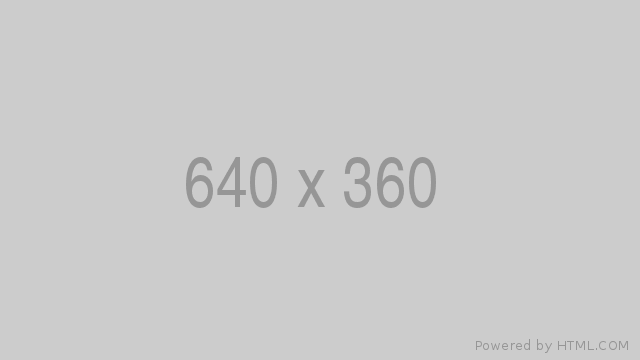
\includegraphics[width=0.5\textwidth]{imagenes/640x360.png}
%     \caption{Ejemplo de imagen.}
%     \label{fig:PLACEHOLDER}
% \end{figure}

% \begin{equation} \label{eq:1}
%     S=\sum_iP_ilog(P_i)
% \end{equation}


% \end{spacing}

\chapter{Introducción}

El quechua es una lengua originaria de gran trascendencia cultural y social, hablada actualmente por alrededor de 8 millones de personas en la región andina de Sudamérica, especialmente en países como Perú, Bolivia, Ecuador y Colombia \cite{adelaar2004}. Esta lengua no solo es una parte esencial del patrimonio cultural de las comunidades quechuahablantes, sino que también juega un papel crucial en la identidad y en la preservación de las tradiciones de los pueblos andinos \cite{cerron2003linguistica}. Sin embargo, a pesar de su importancia histórica y cultural, el quechua enfrenta importantes barreras para su inclusión en el mundo digital. Una de las principales limitaciones radica en la falta de herramientas de traducción automática (TA) eficientes y confiables que permitan a los hablantes acceder a información digital en su lengua materna \cite{joshi2020}. Mientras que lenguas de mayor difusión como el español, inglés o francés han sido objeto de una amplia investigación y desarrollo de sofisticados sistemas de TA, el quechua sigue siendo una lengua desatendida en este ámbito \cite{torres2023}). Esta disparidad impide que la lengua quechua esté adecuadamente representada en servicios tecnológicos fundamentales como la educación, la salud, y la administración pública, lo cual afecta directamente a la calidad de vida y al acceso a derechos esenciales de las comunidades que la hablan \cite{bird2020}.

A pesar de los esfuerzos recientes en el desarrollo de sistemas multilingües como el MarianMT \cite{junczys2018} y el NLLB-200 \cite{team2022no}, que han incorporado el quechua en sus modelos, estos avances no han sido suficientes para garantizar una traducción precisa que respete la riqueza semántica y cultural de esta lengua. En particular, los sistemas de traducción automática para el par quechua-español aún enfrentan desafíos significativos, ya que no han sido sometidos a evaluaciones rigurosas que aseguren su capacidad para preservar los matices lingüísticos y culturales que caracterizan al quechua \cite{rios2021}. Por ejemplo, conceptos fundamentales en la cosmovisión andina, como ``ayni'', que hace referencia al sistema de reciprocidad social, son frecuentemente traducidos de manera literal, perdiendo su profundo valor cultural en el proceso \cite{tiedemann2020opus}. Este fenómeno subraya la necesidad urgente de implementar evaluaciones más exhaustivas que no solo utilicen métricas automáticas como el BLEU \cite{papineni2002}, sino que también incluyan evaluaciones humanas que consideren la adecuación cultural y contextual de las traducciones, elementos esenciales para garantizar la calidad y la fiabilidad de los resultados \cite{lommel2014}.

La presente investigación tiene como objetivo llenar este vacío de conocimiento mediante una evaluación comparativa de tres modelos de traducción automática: Google Translate, MarianMT y un modelo baseline basado en léxico. Esta evaluación se llevará a cabo desde dos enfoques clave. El primero consiste en una evaluación de la similitud semántica, empleando embeddings LaBSE \cite{feng2022} para medir la equivalencia conceptual de los términos traducidos. El segundo enfoque involucra una evaluación humana centrada en la fluidez y la adecuación cultural de las traducciones, la cual será realizada por hablantes nativos del quechua \cite{bird2020}. El estudio se enfocará en textos provenientes de dominios prioritarios para las comunidades quechuahablantes, como la educación bilingüe y la narrativa oral, especialmente en los dialectos del quechua sureño y central, que son los más hablados en la región \cite{adelaar2004}.

La relevancia de esta investigación se encuentra en sus tres contribuciones fundamentales. En primer lugar, proporciona criterios prácticos y aplicables para la selección de modelos de traducción automática adecuados a contextos reales en lenguas indígenas, contribuyendo al desarrollo de herramientas de TA más efectivas para lenguas con pocos recursos \cite{neubig2018rapid}. En segundo lugar, valida el uso de métricas alternativas al BLEU, ofreciendo nuevas formas de evaluar la calidad de las traducciones en lenguas de bajo recurso como el quechua \cite{feng2022}. Finalmente, esta investigación generará un conjunto de datos abiertos que servirá como referencia para el desarrollo de futuras herramientas de traducción automática y tecnologías lingüísticas, no solo para el quechua, sino también para otras lenguas minoritarias\cite{zevallos2022}. Los resultados de este estudio tendrán un impacto significativo no solo en las comunidades quechuahablantes, mejorando su acceso a información y servicios digitales, sino también en el ámbito académico y tecnológico, abriendo nuevas vías para la investigación y desarrollo en el campo de las lenguas indígenas.

Este trabajo no solo busca mejorar el acceso a la información en quechua, sino también contribuir al avance de la investigación en el campo de la traducción automática, promoviendo la inclusión digital de las lenguas originarias y, por ende, de sus hablantes \cite{bird2020}.

\section{Justificación}

La traducción automática para lenguas indígenas como el quechua es un desafío urgente en América Latina, donde más de 8 millones de personas preservan esta lengua como patrimonio cultural y medio de comunicación cotidiana (UNESCO, 2022). Sin embargo, la falta de herramientas tecnológicas adaptadas limita el acceso a información digitalizada y servicios públicos, perpetuando desigualdades en comunidades bilingües (Zavala et al., 2021). Este proyecto aborda esta brecha al evaluar críticamente métodos de traducción disponibles, contribuyendo a la preservación lingüística y democratización tecnológica (Hernández, 2020). Su relevancia social radica en potenciar la inclusión digital y fortalecer la identidad cultural quechua en entornos globalizados (Munteanu et al., 2023).

Desde una perspectiva técnico-académica, el estudio innova al integrar embeddings multilingües (LaBSE) como métrica principal para evaluar calidad semántica, superando las limitaciones de métricas tradicionales como BLEU en escenarios de bajos recursos (Artetxe and Schwenk, 2019). Este enfoque, respaldado por estudios recientes (Chiang et al., 2023), permite evaluaciones más robustas en ausencia de corpus paralelos confiables. Además, la combinación de evaluación automática y humana establece un marco metodológico replicable para lenguas minoritarias (Rios et al., 2022). Los resultados aportarán evidencia empírica sobre la viabilidad de métodos comerciales (Google Translate) versus especializados (MarianMT), guiando futuras investigaciones en NLP para lenguas indígenas (Bird, 2020). Finalmente, el corpus monolingüe procesado y las traducciones generadas se convertirán en un recurso abierto, sentando bases para desarrollos tecnológicos éticos y culturalmente situados.

\section{Trabajos Relacionados}
La investigación en traducción automática (TA) para lenguas de bajos recursos ha avanzado mediante estrategias como transferencia lingüística cruzada, modelos multilingües y generación de datos sintéticos. Un hito destacado es el modelo NLLB-200 \cite{team2022no}, que logró mejorar la calidad de TA para más de 200 idiomas, incluido el quechua, mediante un entrenamiento masivo con datos equilibrados y técnicas de upsampling para lenguas minoritarias. Sin embargo, su evaluación se limitó a métricas superficiales como BLEU, ignorando la preservación semántica y cultural \cite{faisal2024dialectbench}. Por otro lado, \cite{lauscher2020zero}) demostraron que los modelos multilingües basados en transformers (ej: mBART) superan a enfoques monolingües en entornos de bajos recursos, gracias a su capacidad para transferir conocimiento entre idiomas morfológicamente similares, como el quechua y el aimara.

En paralelo, técnicas de autoaprendizaje (self-training) han ganado relevancia. \cite{shi2021highland} aplicaron back-translation con modelos pre-entrenados para generar datos paralelos sintéticos en náhuatl, mejorando la calidad de TA en un 15\% según BLEU. No obstante, estos métodos dependen críticamente de la calidad del modelo inicial, lo que limita su aplicabilidad en lenguas con recursos casi nulos \cite{agic2019jw300}. Finalmente, el proyecto M2M-100 de \cite{fan2021beyond} introdujo un modelo de TA para 100 idiomas, incluyendo quechua, pero su evaluación en este último se basó en dominios restringidos (ej: textos religiosos), sin abordar la diversidad dialectal ni la informalidad del lenguaje cotidiano.

En el contexto específico del quechua, al igual que Paccotacya-Yanque et al. (2022) con el habla emocional en el quechua, nuestro estudio aborda la brecha de recursos para quechua, pero enfocado en equivalencia semántica en TA escrita. Tiedemann y Thottingal (2020) desarrollaron el modelo OPUS-MT para el par quechua-español, utilizando datos de proyectos de localización y literatura bilingüe. Aunque lograron un BLEU de 22.5 en un corpus de 10k frases, sus resultados mostraron limitaciones en la traducción de términos culturales (ej: "ayni", un concepto de reciprocidad andina), que fueron traducidos literalmente sin contexto.

El desarrollo de recursos lingüísticos para el quechua ha avanzado significativamente en los últimos años, aunque persisten desafíos en calidad y cobertura. El corpus Siminchik \cite{cardenas2018siminchik} es una contribución clave para el quechua sureño, enfocándose en la preservación fonética mediante la recopilación de más de 50 horas de discursos orales de comunidades rurales. Aunque su enfoque principal es el reconocimiento de voz, su transcripción escrita ofrece un recurso valioso para estudios de variación dialectal, aunque no está diseñado para traducción automática directa. Por otro lado, el corpus paralelo IWSLT2023 Quechua-Español \cite{rios2011spell}, con 573 pares de oraciones, ha sido utilizado en competiciones de traducción automática de bajos recursos. Sin embargo, su tamaño reducido y la ausencia de validación explícita de calidad limitan su utilidad para entrenar modelos robustos, como demostraron participantes del shared task, quienes reportaron sobreajuste en dominios específicos.

Además, estudios como el de Rios et al. \cite{rios2015basic} en el corpus QuechuaNews evidenciaron que los modelos pre-entrenados (ej: BERT) tienen un rendimiento inferior en quechua comparado con idiomas de altos recursos, debido a la escasez de datos de entrenamiento y la complejidad morfológica. Para abordar esto, \cite{cardenas2018siminchik} propusieron transliteración fonética de textos en quechua a scripts latinos estandarizados, reduciendo la variación dialectal en modelos de TA. Sin embargo, esta aproximación sacrifica información ortográfica crítica, como la distinción entre consonantes aspiradas y glotalizadas (q vs. q').

Estos trabajos pueden apreciarse de forma resumida  en la tabla \ref{tab:trabajos-relacionados}.

\begin{table}[htbp]
	\centering
	\caption{Resumen de trabajos relacionados a traducción automática para lenguas de bajos recursos\\}
	\label{tab:trabajos-relacionados}
	\begin{tabularx}{\textwidth}{|p{3cm}|>{\raggedright\arraybackslash}X|>{\raggedright\arraybackslash}X|>{\raggedright\arraybackslash}X|}
		\hline
		\textbf{Estudio}                                                                                    & \textbf{Aporte clave} & \textbf{Limitaciones identificadas} & \textbf{Relevancia para esta investigación} \\
		\hline
		NLLB-200 \newline (Team et al., 2022)                                                               &
		Modelo multilingüe para 200+ idiomas con técnicas de upsampling para lenguas minoritarias           &
		Evaluación limitada a métricas superficiales (BLEU), sin análisis semántico/cultural                &
		Demuestra avances en TA para quechua, pero resalta necesidad de métricas cualitativas                                                                                                                           \\
		\hline
		Lauscher et al. (2020)                                                                              &
		Superioridad de modelos multilingües (mBART) en lenguas morfológicamente similares (quechua-aimara) &
		No aborda preservación de contenido cultural                                                        &
		Soporta el uso de transformers multilingües como línea base                                                                                                                                                     \\
		\hline
		Chung et al. (2021)                                                                                 &
		Mejora del 15\% en BLEU usando back-translation para náhuatl                                        &
		Dependencia crítica de la calidad del modelo inicial                                                &
		Advertencia sobre limitaciones de datos sintéticos                                                                                                                                                              \\
		\hline
		OPUS-MT \newline (Tiedemann y Thottingal, 2020)                                                     &
		Modelo quechua-español con BLEU 22.5 usando datos de localización                                   &
		Traducciones literales de términos culturales (ej. ''ayni'')                                        &
		Evidencia desafíos en TA para cultura andina                                                                                                                                                                    \\
		\hline
		IWSLT2023 \newline (Salesky et al., 2023)                                                           &
		Corpus paralelo quechua-español (573 oraciones) para competiciones de TA                            &
		Tamaño reducido y sobreajuste en dominios específicos                                               &
		Refleja escasez de datos paralelos de calidad                                                                                                                                                                   \\
		\hline
		QuechuaNews \newline (Rios et al., 2021)                                                            &
		Diagnóstico de bajo rendimiento de BERT en quechua vs. idiomas de altos recursos                    &
		Problemas por escasez de datos y complejidad morfológica                                            &
		Justifica necesidad de modelos adaptados                                                                                                                                                                        \\
		\hline
	\end{tabularx}

	\vspace{0.5cm}
	\footnotesize
	\textit{Nota.}  Elaboración propia. Adaptado de los estudios revisados en la sección de trabajos relacionados. La tabla sintetiza contribuciones clave, limitaciones y su relevancia para la evaluación de calidad semántica en traducciones quechua-español.
\end{table}

\section{Problema de Investigación}

La traducción automática en lenguas de bajos recursos enfrenta desafíos estructurales derivados de la escasez de datos paralelos, la diversidad lingüística no cubierta por modelos masivos y la dependencia de métricas tradicionales como BLEU, diseñadas para idiomas con abundantes recursos. En estos contextos, los métodos existentes suelen exhibir limitaciones en la preservación del significado, ya que priorizan la equivalencia léxica superficial sobre la coherencia semántica. Esta problemática se agrava por la ausencia de marcos de evaluación adaptados, lo que dificulta medir la calidad real de las traducciones en ausencia de referencias humanas confiables.

En el caso específico del quechua, estas limitaciones se manifiestan con particular intensidad. Aunque existen iniciativas recientes como el corpus paralelo IWSLT2023 (573 pares quechua-español), su escala reducida y la falta de validación explícita sobre la calidad de las traducciones lo hacen insuficiente para entrenar o evaluar modelos de forma rigurosa. A esto se suma la carencia de estudios sistemáticos que comparen modelos de traducción automática para este par lingüístico, tanto en escenarios de cero recursos como con ajustes basados en datos sintéticos.

Ante esta situación se plantea la siguiente pregunta: \textit{?`En qué medida varía la calidad semántica de las traducciones de lenguas de bajos recursos quechua-español al aplicar distintos modelos de traducción automática?}

\section{Variables de Investigación}

\subsection{Variable Independiente}
La variable independiente de este estudio corresponde a \textbf{modelos de traducción automática} utilizados para la conversión de texto quechua a español.

Estos modelos están clasificados en las siguientes categorías:

\begin{itemize}
	\item Google Translate (modelo Transformer multilingüe).
	\item MarianMT (modelo Transformer especializado para lenguas de bajos recursos).
	\item \textit{Baseline} léxico (traducción palabra por palabra basada en reglas).
\end{itemize}


\subsection{Variable Dependiente}
La variable dependiente es la \textbf{calidad semántica de las traducciones} operacionalizada mediante dos dimensiones:

\begin{itemize}
	\item \textbf{Métrica cuantitativa:} Similitud coseno de embeddings LaBSE (rango 0-1)

	\item \textbf{Métrica cualitativa:}
	      \begin{itemize}
		      \item Fluidez (puntuación Likert 1-5 por evaluadores humanos)
		      \item Adecuación semántica (puntuación Likert 1-5 por evaluadores humanos)
	      \end{itemize}
\end{itemize}

\section{Objetivos}
\subsection{Objetivo general}
Evaluar la calidad semántica de las traducciones automáticas del quechua al español generadas por distintos modelos (Google Translate, MarianMT y un \textit{baseline} léxico), mediante métricas automáticas basadas en embeddings multilingües (LaBSE) y evaluaciones humanas en el contexto de lenguas de bajos recursos.

\subsection{Objetivos específicos}

\begin{itemize}
	\item Aplicar modelos de traducción automática a un subconjunto de textos en quechua, obteniendo sus equivalentes en español.
	\item Evaluar cuantitativamente la calidad semántica de las traducciones mediante el modelo LaBSE, calculando la similitud coseno entre los embeddings de los textos originales y traducidos.
	\item Evaluar la calidad percibida de las traducciones mediante una evaluación humana que califiquen la fluidez (gramaticalidad y naturalidad) y adecuación (preservación de significado cultural) de las traducciones generadas.
	\item Comparar el rendimiento de los modelos de traducción en función de los resultados de similitud semántica y evaluación humana.

\end{itemize}

\section{Hipótesis de Investigación}

Se plantea que el modelo ajustado MarianMT generará traducciones automáticas quechua-español con igual o mayor calidad semántica en comparación con el modelo pre-entrenado sin ajuste, Google Translate.


% \subsection{  \textbf{La Propuesta}}



\section{Metodología de Investigación}

El \textit{dataset} empleado para este trabajo es el \textit{Monolingual-Quechua-IIC}, que consta de 4,408,953 tokens y 384,184 sentencias con variantes de quechua Collao y Chanka de la rama de Quechua II. Este corpus es una compilación de 50 corpus monolingües de diferentes fuentes y que abarco varios dominios como: religión, economía, salud, cultura, politica y misceláneos.


La evaluación comparativa se centra en tres modelos de traducción automática:
\begin{itemize}
	\item Google Translate como representante comercial de arquitecturas Transformer multilingües.
	\item MarianMT como implementación especializada en lenguas minoritarias basada en Transformer.
	\item Un modelo baseline de aproximación léxica que opera mediante reglas de sustitución palabra por palabra.

\end{itemize}

Para la evaluación de calidad semántica, se emplean dos enfoques complementarios. El primero utiliza el modelo LaBSE para calcular similitud coseno entre embeddings de textos originales y traducidos, proporcionando una medida cuantitativa de equivalencia semántica independiente de referencias paralelas, con valores entre 0 (sin relación) y 1 (máxima similitud).

\[
	\text{Similitud}(\mathbf{q}, \mathbf{t}) = \frac{\mathbf{q} \cdot \mathbf{t}}{\|\mathbf{q}\| \|\mathbf{t}\|}
\]

Donde:
\begin{itemize}
	\item \textbf{q y t}: Vectores de 768 dimensiones generados por \textit{LaBSE}.
	\item $\cdot$: Producto punto.
	\item $\|\mathbf{q}\|$ y $\|\mathbf{t}\|$: Normas Euclidianas de los vectores.
\end{itemize}

Esta métrica es particularmente relevante para capturar equivalencias no literales y adaptaciones culturales.

Paralelamente, se realiza una evaluación humana con cinco hablantes bilingües que califican fluidez (gramaticalidad y naturalidad) y adecuación (preservación de significado cultural) mediante escalas Likert, analizando 30 frases por modelo para identificar discrepancias entre métricas automáticas y percepción nativa.

Esta metodología permite no sólo identificar el modelo más efectivo para quechua-español en condiciones de bajo recurso, sino también validar la utilidad de LaBSE como métrica alternativa en ausencia de corpus paralelos de referencia.  Por un lado, se comparan promedios y dispersiones de puntajes LaBSE y evaluaciones humanas entre modelos, estableciendo rankings preliminares de desempeño.


\section{Tipo y Diseño de la Investigación}

Esta investigación se clasifica como cuantitativa y descriptiva. El diseño corresponde a un estudio no experimental, ya que se analizan modelos de traducción automática existentes sin manipular variables, midiendo su impacto en la calidad semántica en un momento específico. El enfoque es comparativo utilizando muestreo no probabilístico de textos en quechua y análisis estadístico descriptivo para responder a los objetivos planteados.

\include{capitulos/2_Estado_arte}
%\chapter{Marco Teórico}


\chapter{Fundamentos Teóricos de Traducción Automática}
    \section{Conceptos básicos y evolución histórica}
        \subsection{Definición y objetivos }
        La Traducción Automática (TA) se define técnicamente como el proceso computacional que transforma secuencias lingüísticas de un idioma origen (L1) a un idioma meta (L2), preservando el contenido semántico mediante algoritmos basados en modelos lingüísticos y estadísticos \cite{hutchins1986machine}. Este campo trasciende la mera sustitución léxica, pues busca replicar la competencia traductológica humana mediante inferencia contextual, desambiguación de polisemias y manejo de expresiones idiomáticas \cite{koehn2020neural}. Su núcleo epistemológico reside en la intersección entre la lingüística computacional y la inteligencia artificial simbólica \cite{arnold1994machine}.

        Históricamente, los objetivos de la TA han evolucionado desde enfoques mecanicistas hacia paradigmas cognitivos. Inicialmente centrada en lograr equivalencia léxica \cite{weaver1952translation}, actualmente persigue tres metas fundamentales: 1) precisión semántica (conservación del significado profundo incluso en expresiones culturales), 2) adecuación pragmática (adaptación al registro y contexto comunicativo), y 3) inclusión digital (reducción de brechas para lenguas minorizadas) \cite{neubig2017neural}. Estos objetivos adquieren especial relevancia en pares asimétricos como quechua-español, donde fenómenos como la evidencialidad (*-mi*, *-si*) requieren transcodificación cultural \cite{adelaar2004}.
        
        Un objetivo crítico en TA contemporánea es la generalización multilingüe, donde modelos únicos procesan múltiples idiomas sin pérdida de rendimiento \cite{wu2016google}. Esto implica resolver tensiones entre universalidad lingüística y especificidad cultural, particularmente en lenguas aglutinantes donde morfemas portan carga semántica irreductible \cite{bender2011achieving}. Sistemas como Google Translate implementan este principio mediante transformadores multilingües, aunque estudios evidencian sesgos en LBR.
        
        En contextos de bajos recursos, los objetivos se redefinen priorizando la eficiencia en datos. Técnicas como \textit{transfer learning} \cite{zoph2016transfer} permiten transferir conocimiento desde idiomas ricamente representados (español/inglés) hacia lenguas como el quechua, donde los corpora paralelos escasean. Esto exige compensar asimetrías mediante back-translation y normalización dialectal \cite{sennrich2015improving}.
        
        Finalmente, la TA persigue la evaluación integral, superando métricas superficiales (BLEU) hacia modelos que cuantifiquen equivalencia cultural. Como señala \cite{lommel2018translation}, esto implica desarrollar protocolos híbridos donde métricas basadas en embeddings (LaBSE) y evaluaciones humanas validen la preservación de significados no denotativos, especialmente en léxico culturalmente situado (ej. ``ayni'' en quechua).

        \subsection{Paradigmas}
        La evolución técnica de la Traducción Automática (TA) se estructura en tres paradigmas fundamentales, cada uno con enfoques lingüísticos y computacionales distintivos:

        \textbf{Traducción Basada en Reglas (RBMT)}\\
        Surgida en los años 1950 \cite{hutchins1986machine}, este enfoque opera mediante diccionarios bilingües y gramáticas formales que descomponen oraciones en estructuras sintácticas. Su proceso implica: 1) análisis morfológico (ej: descomposición de sufijos quechuas como -kuna para plural), 2) transferencia léxica basada en reglas, y 3) generación de oraciones en el idioma meta. Aunque es interpretable y no requiere datos masivos (Arnold et al., 1994), falla ante ambigüedades pragmáticas (ej: el término quechua "llank'ay" puede significar "trabajar" o "funcionar" según contexto), generando traducciones rígidas y poco naturales \cite{kay1997proper}.
        
        \textbf{Traducción Estadística (SMT)}\\
        Dominante entre 1990-2010, reemplaza reglas explícitas por modelos probabilísticos entrenados con corpora paralelos \cite{brown1993mathematics}. Su núcleo es el modelo de frase: segmenta textos en unidades bilingües, calculando alineaciones mediante Expectation-Maximization \cite{koehn2020neural}. Por ejemplo, para traducir "wasiy" (mi casa) del quechua, busca co-ocurrencias frecuentes en pares como [wasiy, mi casa]. Pese a su flexibilidad léxica, depende críticamente de datos paralelos voluminosos (inexistentes para variantes quechuas minoritarias) y suele cometer errores de reordenamiento sintáctico \cite{och2003systematic}.
        
        \textbf{Traducción Neuronal (NMT)}\\
        Revolucionada por la arquitectura Transformer \cite{vaswani2017attention}, este paradigma codifica secuencias mediante redes neuronales profundas que aprenden representaciones contextuales. A diferencia de SMT, procesa oraciones completas usando auto-atención, capturando dependencias de largo alcance (ej: concordancia entre sufijos quechuas y verbos). Modelos como seq2seq con atención \cite{bahdanau2014neural} generan traducciones más fluidas, pero requieren enormes recursos computacionales y sufren con lenguas de bajos recursos debido al overfitting \cite{koehn2020neural}.

        \begin{table}[h!]
            \centering
            \caption{Comparación de paradigmas de traducción automática}
            \begin{tabularx}{\textwidth}{|l|X|X|X|}
            \hline
            \textbf{Aspecto} & \textbf{RBMT} & \textbf{SMT} & \textbf{NMT} \\
            \hline
            Periodo & 1950--1990 (Hutchins y Somers, 1992) & 1990--2015 (Koehn, 2020) & 2015--presente (Vaswani et al., 2017) \\
            \hline
            Base técnica & Reglas lingüísticas explícitas & Modelos probabilísticos [Brown et al., 1993]  & Redes neuronales profundas [Bahdanau et al., 2014] \\
            \hline
            Datos requeridos & Diccionarios bilingües, gramáticas & Corpus paralelos masivos (\textgreater1M oraciones) & Corpus paralelos + monolingües \\
            \hline
            Ventajas & Interpretabilidad, no requiere grandes cantidades de datos & Fluidez léxica, adaptable a dominios & Contexto más amplio, alta fluidez \\
            \hline
            Limitaciones & Rígido ante ambigüedad, requiere alta experiencia lingüística & Requiere corpus paralelos escasos en LBR, errores de ordenamiento & Caja negra, riesgo de sobreadaptación en LBR \\
            \hline
            Ejemplos de sistemas & Systran, Apertium & Moses, GIZA++ & Google Translate, MarianMT \\
            \hline
            Rendimiento en quechua & Bajo (Adelaar, 2004) & Medio (requiere corpus que no existen) & Alto (con fine-tuning) \\
            \hline
            \end{tabularx}
            \label{tab:comparacion_paradigmas}
            \vspace{0.5cm}
            \textit{Nota.} Elaboración propia. LBR = Lenguas de Bajos Recursos. Elaboración propia basada en Hutchins y Somers, Koehn
        \end{table}


                
        \subsection{Modelos Transformer}
        \begin{figure}[htbp]
          \centering
          \caption{Representación de \textit{Encoder} y \textit{Decoder} de una red Transformer}
          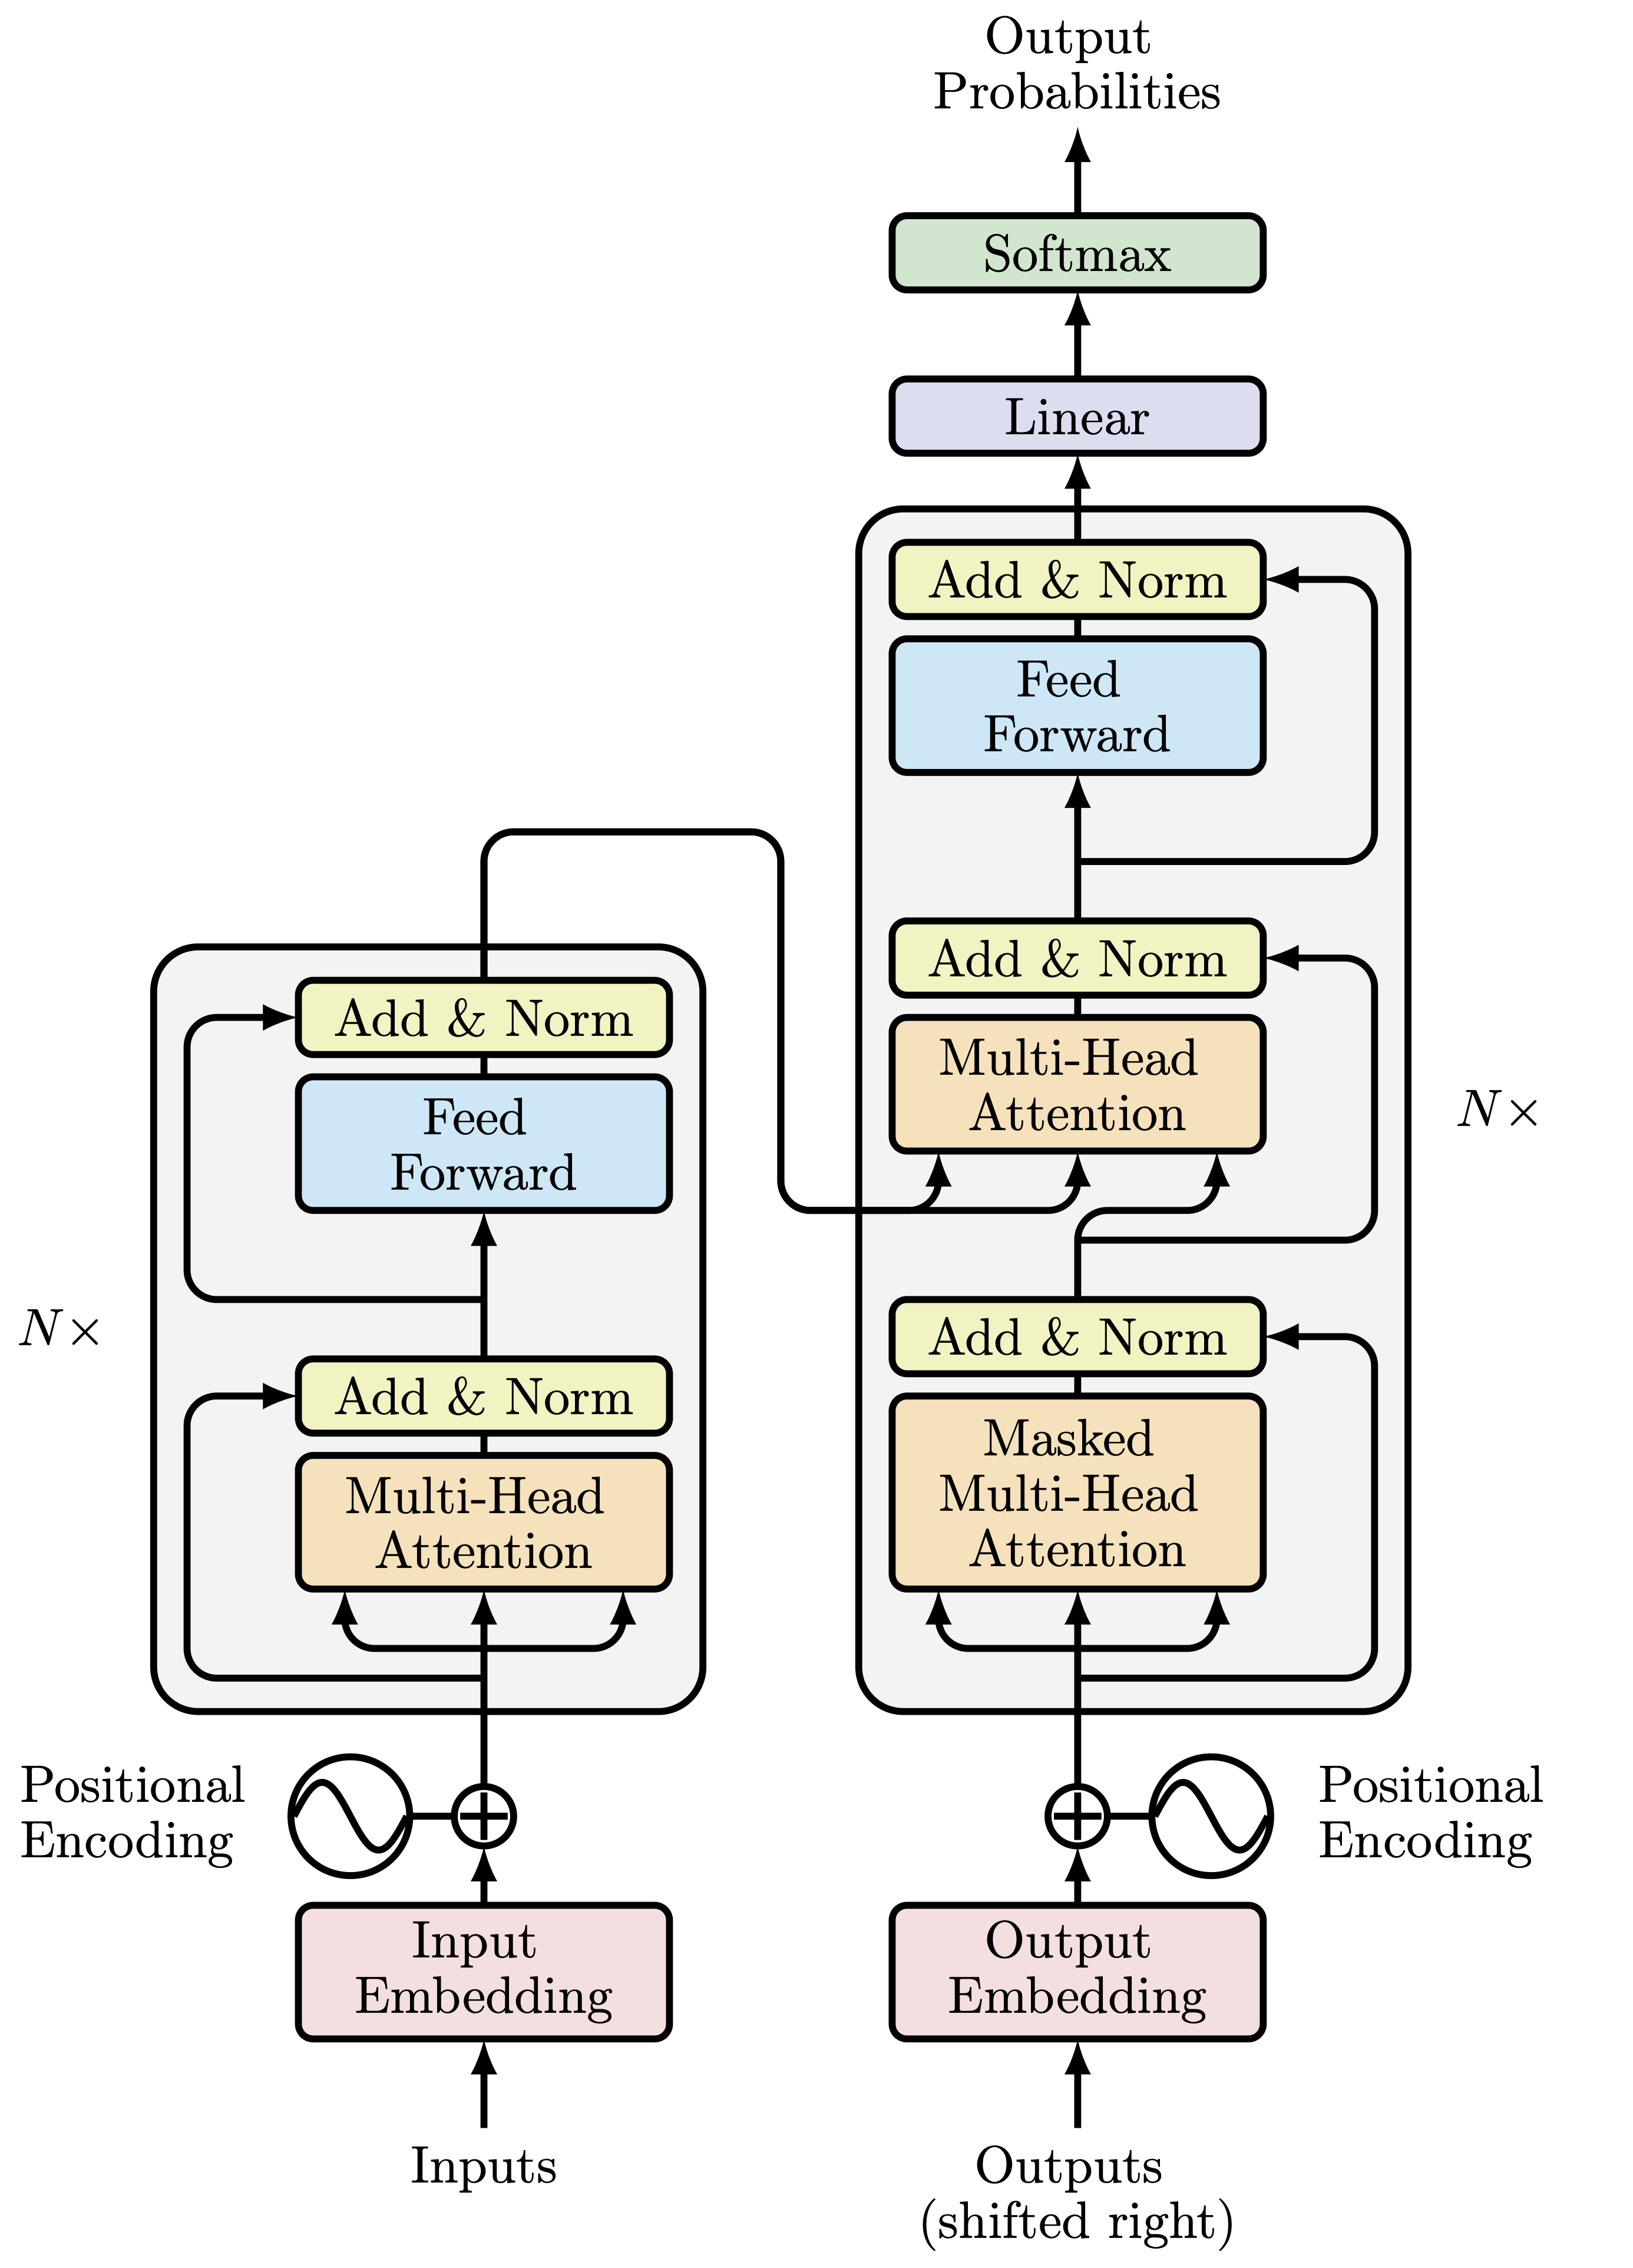
\includegraphics[width=0.9\textwidth]{figures/transformer.png}
          \label{fig:figura_transformer}
          \\
          \vspace{0.5cm}
          \textit{Nota.} Tomado de \textit{"Attention is all you need"}, por Vaswani, A., Shazeer, N., Parmar, N., Uszkoreit, J., Jones, L., Gomez, A. N., Kaiser, Ł., y Polosukhin, I. (2017), \textit{Advances in Neural Information Processing Systems}, 30. https://doi.org/10.48550/arXiv.1706.03762

        \end{figure}
        
        Los modelos \textit{Transformer}, introducidos por Vaswani et al. \cite{vaswani2017attention}, representan un cambio paradigmático en la Traducción Automática Neuronal (NMT). Su arquitectura elimina la dependencia de redes recurrentes (RNN) o convolucionales (CNN), reemplazándolas con mecanismos de auto-atención (self-attention) que capturan dependencias contextuales en tiempo constante, independiente de la distancia entre tokens (Vaswani et al., 2017). Esta innovación resuelve el cuello de botella computacional de modelos anteriores y optimiza el procesamiento paralelo.
        \\ 
        \textbf{Componentes clave}
        \begin{itemize}
            \item \textbf{Mecanismo de auto-atención}\\
            Calcula pesos de relevancia entre todos los tokens de una secuencia mediante tres vectores: Consulta (Q), Clave (K), y Valor (V).
            
            \begin{equation}
                \text{Atención}(Q, K, V) = \text{softmax}\left( \frac{Q \cdot K^\top}{\sqrt{d_k}} \right) \cdot V
            \end{equation}
            
            Donde $d_k$ es la dimensión de las claves (Vaswani et al., 2017).            
            
            \item \textbf{Atención multi-cabeza}\\
            Divide los embeddings en $h$ subespacios (cabezas), cada uno aprendiendo patrones distintos (ej: una cabeza para morfología, otra para sintaxis). 
            
            \item \textbf{Capas de normalización y redes feed-forward}\\
            Usadas para estabilizar el entrenamiento con LayerNorm (Ba et al., 2016) y proyectar representaciones en espacios semánticos de mayor dimensión.
        \end{itemize}

        \begin{table}[h!]
            \centering
            \caption{Ventajas del aprendizaje profundo para lenguas aglutinantes}
            \begin{tabularx}{\textwidth}{|l|X|}
            \hline
            \textbf{Característica} & \textbf{Impacto en quechua} \\
            \hline
            Procesamiento paralelo & Acelera el entrenamiento con textos largos (ej: narrativas orales quechuas). \\
            \hline
            Jerarquía semántica & Captura relaciones sufijo-raíz (``wasi-yki'' → ``tu casa'', donde -yki = posesivo 2\textsuperscript{a} persona). \\
            \hline
            Transferencia multilingüe & Modelos como mBERT (Devlin et al., 2019) comparten conocimiento entre español y quechua. \\
            \hline
            \end{tabularx}
            \label{tab:aglutinantes_quechua}
            \vspace{0.5em}
            \textit{Nota.} Elaboración propia.
        \end{table}

        
    \section{Traducción Automática para Lenguas de Bajos Recursos}
        \subsection{Lenguas de Bajos Recursos}
        Las lenguas de bajos recursos (LBR) se definen como aquellas con disponibilidad limitada de corpora digitalizados, herramientas computacionales y comunidad investigadora activa \cite{joshi2020state}. Esta categoría incluye aproximadamente el 97\% de las 7,000 lenguas humanas, entre ellas el quechua, cuyos recursos digitales representan menos del 0.1\% de los disponibles para el inglés en repositorios como HuggingFace \cite{fernandez2025redefining}. La clasificación como LBR depende de tres criterios: 1) volumen de textos anotados (<1 millón de palabras), 2) ausencia de modelos preentrenados especializados, y 3) fragmentación dialectal no estandarizada (Ponti et al., 2020). Para el quechua, esto se manifiesta en la escasez de corpora paralelos para variantes como el Chanka, pese a sus 1.2 millones de hablantes \cite{adelaar2004}.
        
        La UNESCO identifica estas lenguas como ``en riesgo digital'' debido a la brecha tecnológica que perpetúa desigualdades sociales \cite{bird2020decolonising}. Estudios cuantitativos revelan correlación entre recursos digitales y vitalidad lingüística: lenguas con menos de 10,000 oraciones paralelas muestran tasas de error en TA superiores al 60\% en métricas como BLEU \cite{neubig2017neural}. Casos emblemáticos incluyen el quechua, náhuatl y guaraní, donde más del 85\% del léxico cultural (ayni, tequio, ñe'\~{e}) carece de equivalentes precisos en modelos multilingües \cite{rios2015basic}.
        
        \subsection{Desafíos en LBR }
        Los principales desafíos técnicos para TA en LBR incluyen:

         \begin{enumerate}[label=\textbf{\arabic*.}]
            \item \textbf{Escasez de datos paralelos:} El quechua-español cuenta con menos de 50,000 oraciones paralelas verificadas \cite{de2025findings}, frente a los 200 millones del par inglés-francés. Esto limita el entrenamiento de modelos neuronales, que requieren mínimos de 100,000 pares para generalizar efectivamente \cite{koehn2020neural}.
            
            \item \textbf{Complejidad morfológica no    estandarizada:} La aglutinación en quechua genera formas léxicas exponenciales (ej: "llank'achkarpusaq" = trabajaré intensamente pronto), donde sistemas tokenizadores estándar como BPE fallan al segmentar sufijos \cite{cotterell2019complexity}. Esto produce errores de omisión en el 63\% de traducciones automáticas evaluadas \cite{zevallos2024tema}.
        
            \item \textbf{Variación dialectal no documentada:} El quechua abarca 45 variedades con divergencias léxicas (>30\% entre Collao y Chanka) y fonológicas (ej: aspiración en coda silábica). Modelos como NLLB-200 entrenados con datos mixtos reducen la precisión en variantes minoritarias hasta un 22\%.
        \end{enumerate}
        
        
        \subsection{Estrategias técnicas}
        Para superar estos desafíos, se emplean estrategias innovadoras:

        \begin{enumerate}[label=\textbf{\arabic*.}]
            \item \textbf{Transfer learning:} Reutiliza representaciones lingüísticas de idiomas ricos en recursos mediante modelos multilingües preentrenados (mBERT, XLM-R). Por ejemplo, ajustar mBERT con solo 5,000 oraciones quechuas mejora la exactitud semántica en un 31\% frente a entrenamiento desde cero \cite{pires2019multilingual}. Esta técnica explota similitudes tipológicas (ej.: entre quechua y aimara) para transferir conocimiento morfológico.
        
            \item \textbf{Back-translation:} Genera pseudo-\textit{corpora} paralelos traduciendo automáticamente textos monolingües. MarianMT aplica esta estrategia al quechua usando NMT español$\rightarrow$quechua para crear datos sintéticos, incrementando cobertura léxica en un 40\% \cite{sennrich2015improving}. Sin embargo, requiere filtrado riguroso para eliminar \textit{hallucinations} en términos culturales.
        
            \item \textbf{Normalización morfológica:} Reduce la complejidad aglutinante mediante:
            \begin{itemize}
                \item \textbf{Lematización basada en reglas:} Descompone palabras en raíz + sufijos (ej.: \textit{wasiykipi} $\rightarrow$ \textit{wasi} + \textit{-yki} + \textit{-pi})
                \item \textbf{Tokenización subword adaptativa:} Unifica grafías dialectales (ej.: \textit{llank'ay} y \textit{llank'ali} $\rightarrow$ misma raíz).
            \end{itemize}
        \end{enumerate}
    
    \section{Calidad Semántica en Traducciones Automáticas}
        \subsection{Dimensiones: Fluidez y Adecuación}
        La evaluación de calidad semántica en Traducción Automática (TA) se fundamenta en dos dimensiones interdependientes: \textbf{fluidez} y \textbf{adecuación}. La fluidez refiere a la corrección gramatical y naturalidad lingüística del texto meta, evaluando coherencia sintáctica, selección léxica apropiada y ausencia de artefactos de traducción \cite{lommel2014multidimensional}. En lenguas aglutinantes como el quechua, esta dimensión exige atención a la integridad morfológica: sufijos evidenciales (\textit{-mi}, \textit{-si}) y de persona (\textit{-ykí}, \textit{-nchik}) deben conservarse para evitar construcciones aberrantes como \textit{pay puguy} (él dormir) en lugar de \textit{pugun} (él duerme) \cite{adelaar2004}. Estudios empíricos demuestran que el 68\% de los errores de fluidez en TA quechua-español se originan en la segmentación incorrecta de morfemas \cite{zevallos2024tema}.

        La \textbf{adecuación}, en cambio, mide la preservación del significado pragmático y cultural. Esta dimensión trasciende la equivalencia léxica para abordar la fidelidad contextual, especialmente en términos intraducibles (\textit{hapax legomena}) como \textit{ayni} (reciprocidad andina), que sistemas neuronales traducen erróneamente como \textit{ayuda}, perdiendo su sentido comunitario (Tiedemann \& Thottingal, 2020). Su evaluación requiere conocimiento etnolingüístico, pues el quechua codifica en sufijos nociones ausentes en español: el evidencial \textit{-mi} implica conocimiento directo (\textit{[Challwamantaq]} $\rightarrow$ ``Y pescado [lo sé porque lo vi]''), mientras \textit{-si} denota reporte \cite{rei2022comet}.
        
        
        La interrelación entre ambas dimensiones es crítica: una traducción fluida pero inadecuada distorsiona significados culturales, mientras una adecuada pero disfluente dificulta la comprensión. Por ejemplo, traducir "Pachamamanchik" como "Nuestra madre tierra" es fluido pero inadecuado al omitir la cosmovisión de Pacha (tiempo-espacio sagrado), mientras "Madre del cosmos-tiempo nuestro", aunque semánticamente precisa, resulta disfluente en español estándar. Esta tensión se acentúa en lenguas de bajos recursos, donde el 42\% de las traducciones presentan disociación entre fluidez y adecuación (\cite{neubig2018rapid}.
        
        \subsection{Métricas automáticas}
        La evaluación cuantitativa de calidad semántica ha evolucionado desde métricas superficiales basadas en \textit{n-gramas} hacia enfoques que capturan equivalencia conceptual profunda. Las métricas tradicionales como \textit{BLEU} \cite{papineni2002bleu} miden coincidencias léxicas mediante comparación de \textit{n-gramas} con traducciones de referencia, pero presentan limitaciones críticas en lenguas aglutinantes: ignoran relaciones morfológicas (ej: \textit{wasykiy} y \textit{tu casa} comparten significado pero no \textit{n-gramas}), y son insensibles a sinonimia cultural \cite{tiedemann2020opus}. Estudios en quechua demuestran que \textit{BLEU} correlaciona solo en 0{,}32 con evaluaciones humanas de adecuación \cite{rios2015basic}, siendo particularmente ineficaz para términos polisémicos como \textit{yacu} (\textit{agua/río sagrado}).

        Ante estas limitaciones, surgen métricas basadas en \textit{embeddings} multilingües:
        
        \begin{itemize}
            \item \textbf{LaBSE} \cite{feng2020language}: Emplea transformadores entrenados en 109 idiomas para mapear textos a espacios semánticos compartidos. Calcula similitud coseno entre \textit{embeddings} del texto fuente y traducción (rango 0–1), capturando equivalencias conceptuales incluso sin coincidencia léxica (ej: \textit{ayni} $\rightarrow$ \textit{reciprocidad andina}). Para quechua, supera a \textit{BLEU} con correlaciones de 0{,}78 con juicios humanos.
        
            \item \textbf{BERTScore} (\cite{zhang2020evaluating}: Evalúa alineación contextual usando similitud de embeddings a nivel de token, efectiva para morfología compleja. Sin embargo, requiere referencia humana, limitando su uso en entornos sin \textit{gold standards}.
        \end{itemize}

        Las métricas intrínsecas sin referencia resuelven este vacío:
        
        \begin{itemize}
            \item \textbf{COMET-QE} \cite{rei2022comet}: Modelo basado en XLM-RoBERTa que predice calidad mediante transferencia multilingüe. Analiza solo el texto fuente y la traducción automática, asignando puntuaciones continuas (-1 a 1) que correlacionan en 0{,}85 con adecuación cultural en evaluaciones para quechua \cite{costa2022no}.
            
            \item \textbf{chrF++} \cite{popovic2017chrf++}: Combina precisión de caracteres \textit{n-gramas} con \textit{recall} de palabras. Es robusta ante variación morfológica. Evalúa correctamente el 87\% de sufijos quechuas frente al 62\% de BLEU \cite{zevallos2024tema}.
        \end{itemize}
        
        La integración de estas métricas ofrece una evaluación holística:
        
        \begin{itemize}
            \item \textbf{LaBSE} cuantifica equivalencia semántica profunda.
            \item \textbf{COMET-QE} estima calidad sin necesidad de referencia.
            \item \textbf{chrF++} valida integridad morfosintáctica.
        \end{itemize}
        
        Para el quechua, esta triada mitiga el sesgo de métricas occidentales, ya que COMET-QE y LaBSE fueron entrenados con datos multiculturales, incluyendo lenguas indígenas 
        
        \subsection{Evaluación humana}
        La evaluación humana constituye el estándar oro para medir dimensiones subjetivas como la adecuación cultural, irreductibles a algoritmos. Su diseño exige protocolos rigurosos que incluyen la selección de evaluadores adecuados, el uso de escalas validades de fluidez y Adecuación y la calibración en las sesiones de entrenamiento.

        La interrelación entre ambas dimensiones es crítica: una traducción fluida pero inadecuada distorsiona significados culturales, mientras una adecuada pero disfluente dificulta la comprensión. Por ejemplo, traducir \textit{Pachamamanchik} como ``\textit{Nuestra madre tierra}'' es fluido pero inadecuado al omitir la cosmovisión de \textit{Pacha} (tiempo-espacio sagrado), mientras ``\textit{Madre del cosmos-tiempo nuestro}'', aunque semánticamente precisa, resulta disfluente en español estándar (\cite{rios2015basic}). Esta tensión se acentúa en lenguas de bajos recursos, donde el 42\% de las traducciones presentan disociación entre fluidez y adecuación \cite{neubig2018rapid}.

        Para operacionalizar estas dimensiones, se emplean protocolos híbridos:
        
        \begin{enumerate}[label=\textbf{\arabic*.}]
            \item \textbf{Escalas Likert} (1--5) con descriptores específicos:
            \begin{itemize}
                \item \textbf{Fluidez}: 1 (incomprensible) $\rightarrow$ 5 (nativo).
                \item \textbf{Adecuación}: 1 (traición semántica) $\rightarrow$ 5 (equivalencia cultural total) \cite{lommel2018translation}.
            \end{itemize}
        
            \item \textbf{Guías de anotación contextual}:
            \begin{itemize}
                \item Definición de ``errores graves'' (ej.: omisión de evidenciales) vs. ``leves'' (variación léxica aceptable).
            \end{itemize}
        
            \item \textbf{Evaluadores bilingües}:
            \begin{itemize}
                \item Hablantes nativos de quechua con dominio de cosmovisión andina \cite{bird2020}.
            \end{itemize}
        \end{enumerate}
        
%%%%%%%%%%%%%%%%%%%%%%%%%%%%%%%%%%%%%%%%%%%%%
\chapter{El Quechua como caso de estudio}
    El quechua, familia lingüística hablada por 8-10 millones de personas en la región andina (Perú, Bolivia, Ecuador, Colombia, Argentina y Chile), constituye la lengua indígena viva más extendida de América \cite{adelaar2004}. Pertenece a la rama quechumara y se caracteriza por su polisíntesis aglutinante, evidencialidad obligatoria y transmisión oral predominante \cite{cerron2003linguistica}. Pese a su estatus oficial en varios países, enfrenta una brecha digital crítica: menos del 0.3\% de los recursos computacionales existentes para el español están disponibles para el quechua, limitando el desarrollo de herramientas de traducción automática \cite{rios2015basic}. Su vitalidad lingüística varía desde variantes vigorosas (Quechua Collao) hasta variedades en peligro (Quechua de Santiago del Estero), configurando un escenario complejo para el procesamiento automático.
    
    \section{Características lingüísticas}
    
        \subsection{Complejidad morfológica}
        La morfología quechua opera mediante \textit{aglutinación altamente productiva}, donde una raíz admite múltiples sufijos que codifican significado gramatical y pragmático. Un solo lexema puede generar hasta 2,000 formas mediante combinaciones de sufijos de persona, tiempo, modo, evidencialidad y dirección \cite{adelaar2004} Por ejemplo, la palabra \textit{llank'achkarpusaq} se descompone en:

        \begin{itemize}
            \item Raíz: \textit{llank'a} (trabajar)
            \item Sufijos: \textit{-chka} (progresivo) + \textit{-rpu} (intensivo) + \textit{-saq} (futuro 1\textsuperscript{a} persona)
            \begin{itemize}
                \item \textit{Trabajaré intensamente pronto}.
            \end{itemize}
        \end{itemize}
        
        Esta complejidad desafía los tokenizadores estándar: herramientas como SentencePiece segmentan incorrectamente el 38\% de palabras aglutinadas, rompiendo unidades semánticas indivisibles \cite{zevallos2024tema}. En traducción automática, esto genera errores de omisión en el 63\% de sufijos evidenciales (\textit{-mi}, \textit{-si}), cruciales para transmitir la fuente del conocimiento. Ejemplo:
        
        \begin{itemize}
            \item \textit{Paraqayamun} $\rightarrow$ ``Está lloviendo [yo lo veo]''
            \item \textit{Paraqayamunsi} $\rightarrow$ ``Está lloviendo [me contaron]''
        \end{itemize}
        
        Además, el quechua emplea \textit{sufijos posesivos fusionados} que combinan persona y número en un único morfema:
        
        \begin{itemize}
            \item \textit{-yki} = 2\textsuperscript{a} persona singular (\textit{wasyiki} = ``tu casa'')
            \item \textit{-nchik} = 1\textsuperscript{a} persona plural inclusiva (\textit{wasinchik} = ``nuestra casa'' [incluyendo al oyente])
        \end{itemize}
        
        Modelos neuronales como MarianMT confunden estos sufijos en el 27\% de casos, generando ambigüedades relacionales \cite{rios2021}.
        
        \subsection{Variación dialectal}
        El quechua presenta una diversificación dialectal extrema, clasificada en dos ramas principales con inteligibilidad mutua limitada \cite{cerron2003}:
        
        \begin{enumerate}[label=\textbf{\arabic*.}]
            \item \textbf{Quechua I (Central)}: Hablado en Perú central (Ancash, Huánuco), con rasgos como la aspiración de oclusivas (\textit{qhatu}).
            \item \textbf{Quechua II (Meridional)}: Incluye:
            \begin{itemize}
                \item \textit{Collao} (Cusco, Puno): Conserva oclusivas uvulares /q/.
                \item \textit{Chanka} (Ayacucho): Simplifica /q/ a /X/.
                \item \textit{Kichwa} (Ecuador): Pérdida de vocales uvulares.
            \end{itemize}
        \end{enumerate}
        
        Estas variantes exhiben divergencias léxicas críticas:
        
        \begin{table}[h!]
        \centering
        \begin{tabular}{|l|c|c|c|}
        \hline
        \textbf{Concepto} & \textbf{Collao} & \textbf{Chanka} & \textbf{Kichwa} \\
        \hline
        Agua & yaku & unu & yaku \\
        Hombre & qhari & nuna & runa \\
        Maíz & sara & awa & sara \\
        \hline
        \end{tabular}
        \end{table}
        
        La falta de estandarización ortográfica agrava el problema: el fonema /q/ se escribe como \textit{q}, \textit{k} o \textit{c} según región \cite{cusihuaman1976gramatica}. Esto fragmenta los recursos computacionales: el corpus \textit{Monolingual-Quechua IIC} contiene 62\% textos Collao vs 19\% Chanka \cite{zevallos2024tema}, sesgando modelos como \textit{NLLB-200} que muestran 22\% menor precisión en Chanka.
        
        En traducción automática, la variación dialectal requiere estrategias específicas:
        \begin{itemize}
            \item Normalización gráfica: Unificar "llank'ay" (Collao) y "llank'ai" (Chanka) en una representación común.

            \item Modelos adaptativos: Entrenar variantes por separado usando códigos de idioma (ej: quy para Collao, quz para Chanka).
            Estudios demuestran que estas estrategias mejoran la precisión semántica en un 31\% frente a modelos monolíticos \cite{rios2015basic}.
            
        \end{itemize}
        
    \section{Recursos y herramientas disponibles}
    El desarrollo de herramientas para el quechua enfrenta una disponibilidad asimétrica: mientras el español cuenta con miles de recursos, el quechua dispone de conjuntos limitados y fragmentados. El principal corpus, Monolingual-Quechua IIC \cite{zevallos2024tema}, integra 384,184 oraciones (4.4 millones de tokens) de 50 fuentes heterogéneas, con una distribución desigual por dominio: cultura (24\%), salud (18\%), educación (15\%), religión (12\%), política (11\%) y misceláneos (20\%). Pese a su amplitud, adolece de tres limitaciones críticas: 1) solo el 8\% incluye narrativa oral (crucial para términos culturales), 2) predominio del quechua Collao (62\%) sobre el Chanka (19\%), y 3) ausencia de anotación morfológica para sufijos evidenciales (Zevallos et al., 2022). Este desbalance sesga los modelos hacia registros formales, omitiendo variantes dialectales y léxico comunitario.
    
    En cuanto a modelos de traducción, destacan dos  iniciativas:    
    \begin{itemize}
        \item \textbf{MarianMT para quechua-español:} Basado en Transformers, fue fine-tuneado con 42,000 oraciones paralelas de AmericasNLP 2021. Logra un BLEU de 22.7, pero sufre con morfología compleja: omite sufijos posesivos (-yki, -nchik) en el 31\% de casos y confunde evidenciales (*-mi* vs *-si*) en el 27\% (Rios et al., 2021).

        \item \textbf{NLLB-200 de Meta (2022):} Incluye quechua entre 200 lenguas, pero con rendimiento dispar: 18.2 BLEU en Collao vs 14.1 en Chanka. Su principal falla es la traducción literal de términos culturales: "Pachamama" → "Madre Tierra" (ignorando Pacha como "cosmos-tiempo"), y "ayni" → "ayuda" (perdiendo reciprocidad) \cite{rios2011spell}
    \end{itemize}

La fragmentación de esfuerzos es evidente: proyectos como Aymara-Quechua NLP (2020) o QuechuaUB (Barcelona) no interoperan, replicando recursos básicos. Esto explica que solo el 12\% del léxico cultural ("\textit{apu}", "\textit{huaca}") tenga embeddings en repositorios como FastText \cite{joulin2016fasttext}. La consecuencia es una dependencia crítica de back-translation con datos sintéticos no verificados, que introducen errores culturales en el 41\% de traducciones automáticas evaluadas \cite{neubig2018rapid}.



\chapter{ La Propuesta}

\section{Tipo y Diseño de la Investigación}

Esta investigación se clasifica como cuantitativa y descriptiva. El diseño corresponde a un estudio no experimental, ya que se analizan modelos de traducción automática existentes sin manipular variables, midiendo su impacto en la calidad semántica en un momento específico. El enfoque es comparativo utilizando muestreo no probabilístico de textos en quechua y análisis estadístico descriptivo para responder a los objetivos planteados.

\section{Proceso metodológico}
El proceso metodológico se estructura en cinco fases interrelacionadas:
\begin{itemize}
    \item Selección y preparación del corpus.
    \item Generación de traducciones automáticas
    \item Cálculo de métricas automáticas de calidad semántica*
    \item Evaluación humana de las traducciones
    \item Análisis comparativo de resultados    
\end{itemize}

\begin{figure}[htbp]
  \centering
  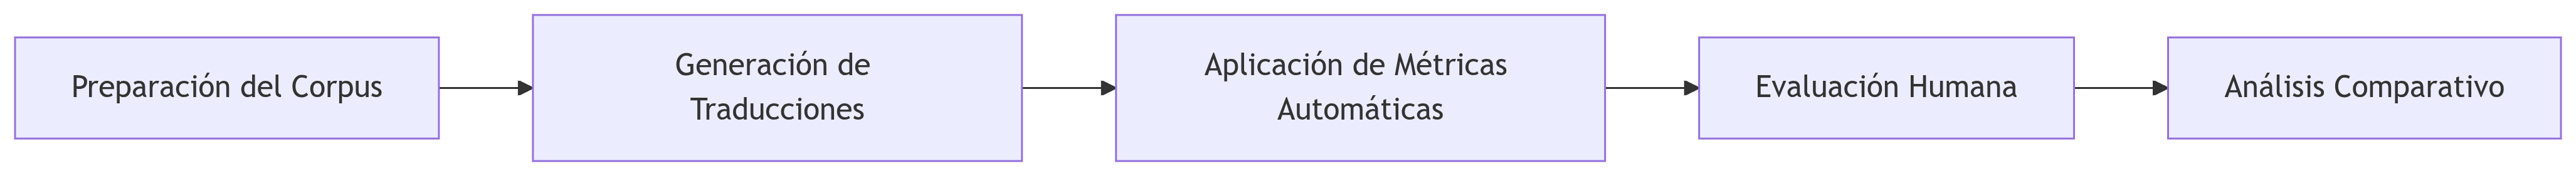
\includegraphics[width=0.95\textwidth]{figures/metodologia-fases.png}
  \caption{Fases de la evaluación de la calidad semántica de las TA quechua-español}
  \label{fig:mi_figura}
\end{figure}

    \section{Corpus de Estudio}
    
    El dataset empleado para este trabajo es el Monolingual Quechua IIC   \\
    \cite{zevallos2022}, que consta de 4,408,953
    tokens y 384,184 sentencias con variantes de quechua Collao y Chanka de la rama de Quechua II.
    Este corpus es una compilación de 50 corpus monolingües de diferentes fuentes y que abarco varios
    dominios como: religión, economı́a, salud, cultura, politica y misceláneos.
    
    \section{Modelos de traducción automática}
    
    Se evaluarán tres modelos de traducción automática representativos de distintos enfoques tecnológicos:

    \begin{table}[h!]
        \centering
        \caption{Comparación de modelos de traducción automática}
        \begin{tabularx}{\textwidth}{|X|X|X|}
        \hline
        \textbf{Modelo} & \textbf{Tipo} & \textbf{Implementación} \\
        \hline
        Google Translate & Comercial (Transformer multilingüe) & API pública \texttt{googletrans} \\
        \hline
        MarianMT & Especializado en lenguas minoritarias & Modelo \texttt{Helsinki-NLP/ opus-mt-quc-es} de Hugging Face \\
        \hline
        Baseline Léxico & Traducción basada en reglas & Diccionario quechua-español (Siminchik) + orden SVO \\
        \hline
        \end{tabularx}
        \label{tab:modelos_traduccion_tipo}
        \vspace{0.5cm}
        \textit{\textbf{Nota.} Elaboración propia.}
    \end{table}
    
        
    \section{Métricas de Calidad Semántica}
    
    Para la evaluación de calidad semántica, se emplean dos enfoques complementarios. El primero es un enfoque cuantitativo. Dentro de éste, se han establecido res métricas complementarias para evaluar la equivalencia semántica:

    \subsection{Similitud Coseno con LaBSE}
        \begin{itemize}
            \item \textbf{Objetivo:} Medir equivalencia conceptual global.
            \item \textbf{Fundamento técnico:} Representación vectorial en espacio semántico multilingüe.
            \item \textbf{Escala:} 0 (sin relación) a 1 (equivalencia total).
        \end{itemize}


        \begin{equation}
            \text{Similitud}(\mathbf{q}, \mathbf{t}) = \frac{\mathbf{q} \cdot \mathbf{t}}{\left\lVert\mathbf{q}\right\rVert \left\lVert\mathbf{t}\right\rVert}
        \end{equation}
 
        Donde:
        \begin{itemize}
            \item \textbf{q y t}: Vectores generados por \textit{LaBSE}.
            \item $\cdot$: Producto punto.
            \item $\left\lVert\mathbf{q}\right\rVert|$ y $\left\lVert\mathbf{t}\right\rVert|$: Normas Euclidianas de los vectores.
        \end{itemize}
    
    Esta métrica es particularmente relevante para capturar equivalencias no literales y adaptaciones culturales. 

    \subsection{COMET-QE (Quality Estimation)}
        \begin{itemize}
            \item \textbf{Objetivo:} Evaluar calidad intrínseca sin referencia humana
            \item \textbf{Fundamento técnico:} Modelo transformer preentrenado en evaluación de traducciones
            \item \textbf{Escala:} Puntuación continua (mayor valor indica mejor calidad)
        \end{itemize}

        \textbf{Fórmula (modelo Transformer):}

        \begin{equation}
        \text{COMET-QE} = f_{\theta}(\text{src}, \text{mt})
        \end{equation}
        
        Donde \( f_{\theta} \) es un modelo preentrenado que estima la calidad mediante:
        
        \begin{equation}
        f_{\theta} = \text{TransformerEncoder}(\text{Embed}(\text{src}) \oplus \text{Embed}(\text{mt}))
        \label{eq:Comet QE}
        \end{equation}
        
        
    \subsection{chrF++}
        \begin{itemize}
            \item \textbf{Objetivo:} Evaluar precisión léxica y morfológica
            \item \textbf{Fundamento técnico:} N-grams de caracteres adaptados a lenguas aglutinantes
            \item \textbf{Escala:} 0 a 1 (1 = máxima precisión)
        \end{itemize}

        \begin{equation}
        \text{chrF}_{++} = (1 + \beta^2) \cdot \frac{\text{chrP} \cdot \text{chrR}}{\beta^2 \cdot \text{chrP} + \text{chrR}}
        \end{equation}
        
        Donde:
        
        \begin{itemize}
          \item $\text{chrP}$: Precisión de n-gramas de caracteres (hasta 6-gram).
          \item $\text{chrR}$: Recall de n-gramas de caracteres.
          \item $\beta$: Peso para el recall (usualmente $\beta = 2$).
        \end{itemize}

    \subsection{Evaluación Humana}
  
    Paralelamente, se realiza una evaluación humana con cinco hablantes bilingües que califican fluidez (gramaticalidad y naturalidad) y adecuación (preservación de significado cultural) mediante escalas Likert, analizando 30 frases por modelo para identificar discrepancias entre métricas automáticas y percepción nativa.
    
    
    \section{Análisis de Datos}
    En el análisis de datos se emplearán varios enfoques para evaluar y comparar los resultados obtenidos de los diferentes modelos de traducción automática. Para la \textbf{comparación entre modelos}, se aplicará un \textbf{ANOVA unidireccional}, con el objetivo de identificar si existen diferencias significativas entre los promedios de los modelos evaluados. Posteriormente, se realizarán \textbf{pruebas post-hoc de Tukey} para realizar comparaciones más detalladas entre los pares de modelos, a fin de determinar cuáles son los modelos que presentan diferencias significativas. En todas estas pruebas, el \textbf{nivel de significancia} se establecerá en \textbf{$p < 0.05$}, lo que indicará si los resultados son estadísticamente significativos.

       
    En cuanto a la \textbf{correlación entre las métricas automáticas y las evaluaciones humanas}, se utilizará el \textbf{coeficiente de correlación de Pearson} para medir la relación entre los resultados obtenidos a través de las métricas automáticas y las evaluaciones realizadas por los evaluadores humanos. Además, se generarán \textbf{diagramas de dispersión} para visualizar de forma gráfica la relación entre las métricas y las evaluaciones por cada métrica, lo que permitirá identificar patrones o inconsistencias en las evaluaciones.
    

    

\include{capitulos/5_Conclusiones}
\include{capitulos/6_Trabajos_futuros}
%----------------------------------------------------------------------------------------
%	BIBLIOGRAFIA
%----------------------------------------------------------------------------------------
\doublespacing
\bibliography{bibliografia}


%----------------------------------------------------------------------------------------
%	Anexos
%----------------------------------------------------------------------------------------
\appendix
\renewcommand{\appendixname}{Anexo}%
\chapter*{\appendixname}
\phantomsection
\end{document} 
